% Ubah kalimat sesuai dengan judul dari bab ini
\chapter{TINJAUAN PUSTAKA}

% Ubah konten-konten berikut sesuai dengan yang ingin diisi pada bab ini

\section{Pengolahan Citra dan Video}

% % Contoh input gambar dengan format *.jpg
% \begin{figure} [ht] \centering
%   % Nama dari file gambar yang diinputkan
%   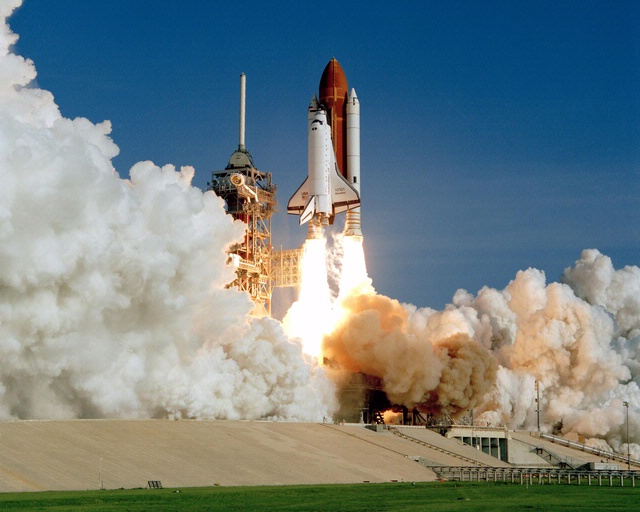
\includegraphics[scale=0.3]{gambar/space-shuttle.jpg}
%   % Keterangan gambar yang diinputkan
%   \caption{Peluncuran pesawat luar angkasa Discovery \citep{DiscoverySpaceShuttle}}
%   % Label referensi dari gambar yang diinputkan
%   \label{fig:SpaceShuttle}
% \end{figure}

Citra adalah sebuah gambar dua dimensi yang diciptakan dari kombinasi antara titik, garis, bidang, dan warna.
Pada pengolahan Citra, citra yang digunakan merupakan citra digital.
Sedangkan, video merupakan kumpulan citra yang saling berhubungan.
Pengolahan Citra dan Video merupakan suatu usaha untuk melakukan transformasi citra/gambar menjadi citra lain dengan menggunakan algoritma-algoritma khusus.
Dengan menggunakan algoritma-algoritma ini masalah-masalah seperti \textit{noise} dan \textit{distortion} pada saat pemrosesan dapat dihindari.

% Contoh penggunaan referensi dari gambar yang diinputkan
% \emph{Discovery}, Gambar \ref{fig:SpaceShuttle}, merupakan \lipsum[17][1-9]

\section{Visi Komputer}

Visi komputer adalah sebuah teknologi yang menggabungkan kamera, komputasi lokal atau awan, perangkat lunak, dan kecerdasan buatan sehingga mesin/komputer mampu untuk melakukan penglihatan layaknya manusia dan melakukan identifikasi objek \cite{vision}.

  \subsection{Ekstraksi Fitur}

  % Contoh penggunaan referensi dari pustaka
  % Newton \citep{Newton1687} pernah merumuskan bahwa \lipsum[19]
  % Contoh penggunaan referensi dari persamaan
  % Kemudian menjadi persamaan seperti pada persamaan \ref{eq:FirstNewtonLaw}.

  % % Contoh pembuatan persamaan
  % \begin{equation}
  %   % Label referensi dari persamaan yang dibuat
  %   \label{eq:FirstNewtonLaw}
  %   % Baris kode persamaan yang dibuat
  %   \sum \mathbf{F} = 0\; \Leftrightarrow\; \frac{\mathrm{d} \mathbf{v} }{\mathrm{d}t} = 0.
  % \end{equation}
  Ekstraksi fitur didapat dengan memproyeksikan fitur ke dalam dimensi yang lebih rendah.
  Pada pengolahan citra dan video, ekstraksi fitur bertujuan untuk menemukan atribut pola-pola yang diinginkan agar bisa diklasifikasikan atau diolah nantinya.
  Ekstraksi fitur dapat dilaksanakan karena beberapa alasan:

    \begin{enumerate}[nolistsep]
      
      \item Mengurangi data masukan (sehingga mempercepat proses dan mengurangi kebutuhan data).

      \item Menyediakan sekumpulan fitur yang relevan untuk proses klasifikasi.

      \item Mengurangi redudansi.

      \item Menemukan variabel fitur yang menjelaskan data.

      \item Menghasilkan representasi dalam dimensi yang lebih kecil dengan sedikit informasi yang hilang.

    \end{enumerate}

  \subsection{Pemilihan Fitur}

  Selain Ekstraksi Fitur, terdapat pemilihan fitur yang memiliki tujuan berbeda dengan ekstraksi fitur, yaitu untuk memilih sejumlah fitur yang ada dari fitur-fitur yang terdapat pada citra.
  Terkadang fitur dari suatu citra tidak berhubungan secara langsung, namun fitur tersebut masih menggambarkan citra asal.

\section{\textit{Machine Learning}}
\textit{Machine Learning} merupakan salah satu cabang teknologi yang menerapkan penggunaan \textit{Artificial Intelligence}.
\textit{Machine Learning} pertama kali diperkenalkan oleh Thomas Bayes, Adrien-Marie Legendre, dan Andrey Markov pada sekitar tahun 1920.
Dengan menggunakan fundamental \textit{Machine Learning} yang diciptakan oleh ilmuwan-ilmuwan tersebut, \textit{Artificial Intelligence} kini dapat berkembang sampai dapat mengalahkan pemain catur profesional.

Dengan berkembangnya \textit{Machine Learning} menjadikan tugas-tugas yang dilakukan oleh \textit{Machine Learning} ini pun semakin beragam.
Beberapa contoh dari tugas yang dapat dilakukan oleh \textit{Machine Learning} adalah validasi data, menemukan pola-pola tertentu dari sumber data yang besar, mengklasifikasi grup dan objek berdasarkan kesamaan pola.
  
  \subsection{\textit{Supervised Learning}}

    \begin{figure}[hbt!] \centering
      % Nama dari file gambar yang diinputkan
      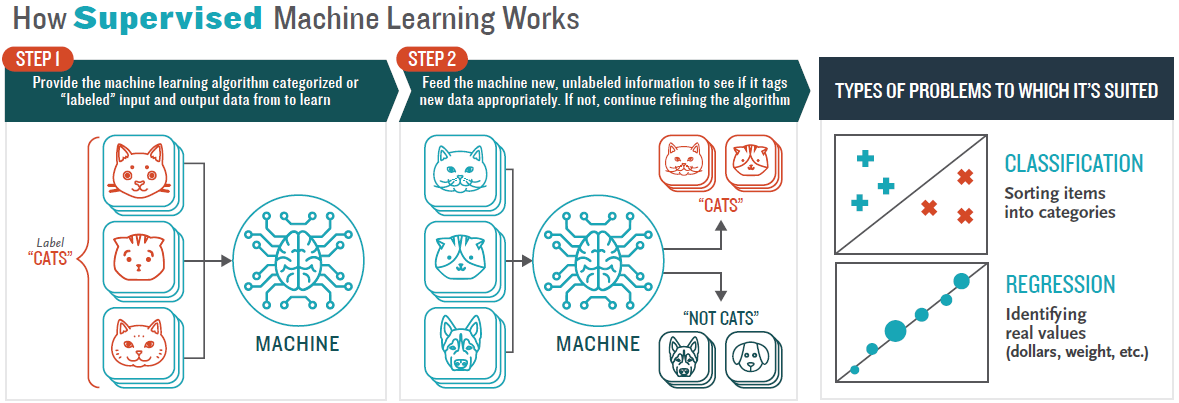
\includegraphics[scale=0.3]{gambar/supervised.png}
      % Keterangan gambar yang diinputkan
      \caption{\textit{Supervised Learning} \cite{booz}}
      % Label referensi dari gambar yang diinputkan
      \label{fig:supervisedLearning}
    \end{figure}

  \textit{Supervised Learning} jika diartikan secara harfiah adalah pembelajaran yang diawasi.
  Disini pengawasan dilakukan oleh orang yang melakukan \textit{training} kepada label di setiap datanya seperti pada gambar \ref{fig:supervisedLearning}.

  Pada gambar \ref{fig:supervisedLearning}, masing-masing gambar kucing diberi label \textbf{“CATS”} dan yang bukan kucing (“anjing”, ”beruang”, dsb.) diberi label \textbf{“NOT CATS”}.
  Ketika gambar baru dimasukkan setiap label akan dibandingkan sampai selesai dan yang memiliki probabilitas lebih banyak akan diambil sebagai prediksi akhir.

  Pada pendekatan \textit{Supervised Learning}, terdapat masukan dan luaran yang dapat dibuat menjadi hubungan matematis.
  \textit{Supervised Learning} cocok untuk digunakan untuk prediksi di mana sudah ada contoh data yang lengkap sehingga pola yang terbentuk adalah hasil pembelajaran dari data lengkap tersebut.
  Beberapa algoritma yang termasuk dalam supervised learning adalah:

    \begin{enumerate}[nolistsep]
      
      \item Regresi Linear

      \item Analisis Deret Waktu

      \item \textit{Decision Tree} dan \textit{Random Forest}

      \item Klasifikasi Naive Bayes

      \item Klasifikasi \textit{k-Nearest Neighbors (k-NN)}

      \item Jaringan Saraf Tiruan

      \item \textit{Support Vector Machine (SVM)}

    \end{enumerate}

  \subsection{\textit{Unsupervised Learning}}

    \begin{figure}[hbt!] \centering
      % Nama dari file gambar yang diinputkan
      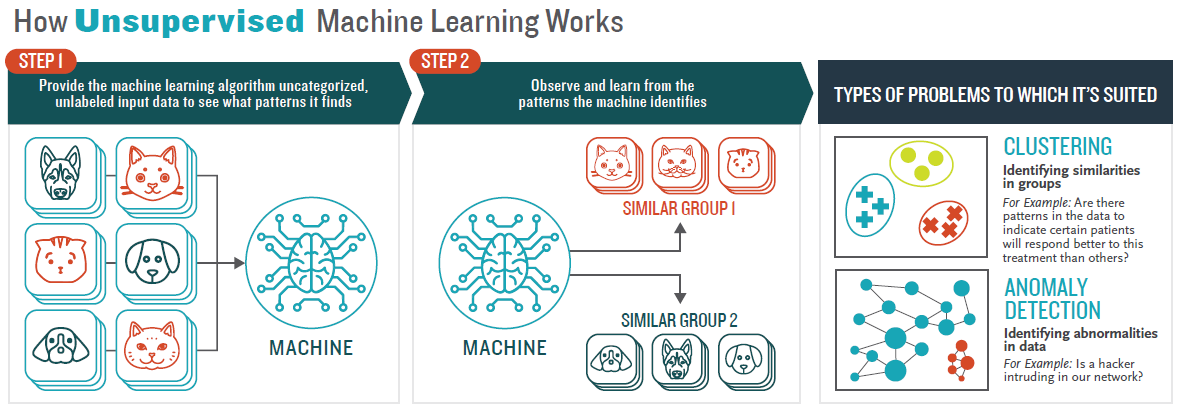
\includegraphics[scale=0.3]{gambar/unsupervised.png}
      % Keterangan gambar yang diinputkan
      \caption{\textit{Unsupervised Learning} \cite{booz}}
      % Label referensi dari gambar yang diinputkan
      \label{fig:unsupervisedLearning}
    \end{figure}

  Jika dibandingkan dengan metode \textit{Supervised Learning}, \textit{Unsupervised Learning} tidak membutuhkan adanya label sebagai dasar prediksi melainkan menggunakan kesamaan atribut-atribut yang dimiliki oleh data tersebut.
  Jika atribut-atribut tersebut memiliki kesamaan maka data tersebut akan di cluster menjadi satu.
  Sebagai contoh dapat dilihat pada gambar \ref{fig:unsupervisedLearning}:

  Pada gambar \ref{fig:unsupervisedLearning} dapat dilihat bahwa disediakan gambar-gambar yang tidak memiliki label ke dalam algoritma \textit{Machine Learning}.
  Setelah itu \textit{Artificial Intelligence} akan memisahkan gambar mana yang memiliki kesamaan di dalam klaster.
  Klaster yang ada merupakan hasil akhir klasifikasi yang dilakukan.

  Namun unsupervised learning tidak memiliki hasil spesifik layaknya pada supervised learning.
  Hal ini dikarenakan tidak adanya label dasar (\textit{ground truth}).
  Beberapa algoritma yang digunakan di \textit{Unsupervised Learning}:

    \begin{enumerate}[nolistsep]
      
      \item \textit{Clustering}

      \item \textit{Anomaly Detection}

      \item \textit{Association Discovery}

    \end{enumerate}

\section{\textit{Deep Learning}}

  \begin{figure}[hbt!] \centering
    % Nama dari file gambar yang diinputkan
    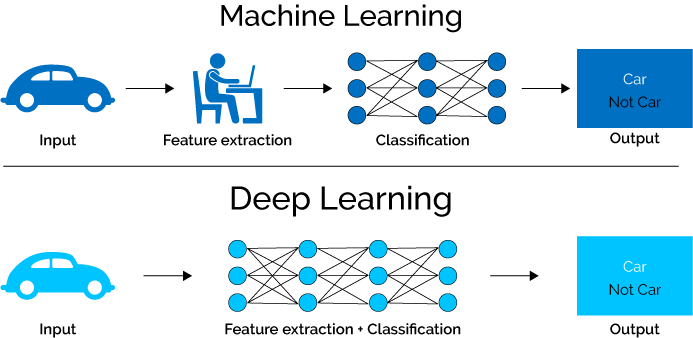
\includegraphics[scale=0.3]{gambar/deeplearning.png}
    % Keterangan gambar yang diinputkan
    \caption{\textit{Deep Learning} \cite{xenonstack_2021}}
    % Label referensi dari gambar yang diinputkan
    \label{fig:deeplearning}
  \end{figure}

\textit{Deep Learning} (Pembelajaran Mendalam) merupakan bagian yang dalam dari \textit{Machine Learning} yang cara kerjanya terinspirasi cara kerja otak manusia, yaitu menggunakan hubungan dari \textit{neuron-neuron} yang ada di dalam otak \cite{deepAI}.
Salah satu kelebihan dari metode \textit{Deep Learning}, pemilihan dan ekstraksi fitur dilakukan sepenuhnya oleh sistem sehingga kita tidak perlu repot untuk memilih fitur apa saja yang akan digunakan.
Hal tersebut bisa kita lihat seperti ada di gambar \ref{fig:deeplearning}.

Beberapa teknik \textit{Deep Learning} yang populer di antaranya adalah \cite{brownlee_2020}:

  \begin{enumerate}[nolistsep]
        
    \item \textit{Multilayer Perceptron Networks}

    \item \textit{Convolutional Neural Networks}

    \item \textit{Long Short-Term Memory Recurrent Neural Networks}

  \end{enumerate}

\section{Python}

  \begin{figure}[hbt!] \centering
    % Nama dari file gambar yang diinputkan
    
\includegraphics[scale=0.3]{gambar/python.png}
    % Keterangan gambar yang diinputkan
    \caption{Logo Python \cite{psf}}
    % Label referensi dari gambar yang diinputkan
    \label{fig:logoPython}
  \end{figure}

Python adalah sebuah bahasa pemrograman \textit{general purpose} dan memiliki berbagai macam paradigma yang dibuat oleh Guido van Rossum dan dirilis pertama pada tahun 1991.
Dewasa ini bahasa pemrograman ini sangat populer karena sering digunakan di dalam penelitian \textit{Deep Learning}.

\section{Cloud Computing}

\textit{Cloud Computing} atau jika diterjemahkan ke bahasa Indonesia sebagai komputasi awan, adalah cara penggunaan sumber daya atau fasilitas komputasi yang meliputi \textit{server}, \textit{storage}, \textit{database}, jaringan atau \textit{networking}, perangkat lunak, analisis, dan kecerdasan internet dengan premis inovasi yang lebih cepat, fleksibel, dan ekonomis.
Layanan \textit{Cloud Computing} yang populer untuk sekarang yaitu Google Cloud, Microsoft Azure, dan AWS.